\section{Use-case analysis}

\subsection{The whole system}

\textit{Figure 2.1} serves as a foundational element in our analysis, offering a high-level depiction of the primary actors and their associated functionalities within the adoption application system.

\begin{figure}[H]
  \centering
  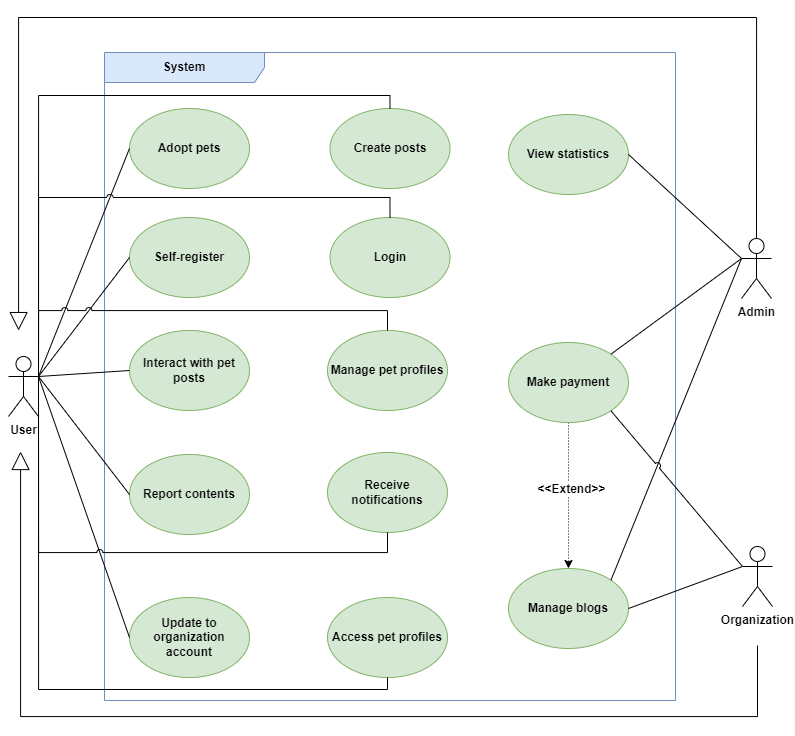
\includegraphics[width=0.6\textwidth]{Figures/system_ucd.png}
  \caption{Use-case diagram of the whole system}
  \label{fig:whole-system_activity_diagram}
\end{figure}

The comprehensive view Figure 1 provided sets the stage for a detailed exploration of each actor's specific use cases, providing a comprehensive understanding of the system's functionalities. As we proceed with our analysis, we will delve into the intricate details of each key function, exploring their roles and contributions to the overall functionality of the adoption application system.

\subsection{Login}

\begin{figure}[H]
  \centering
  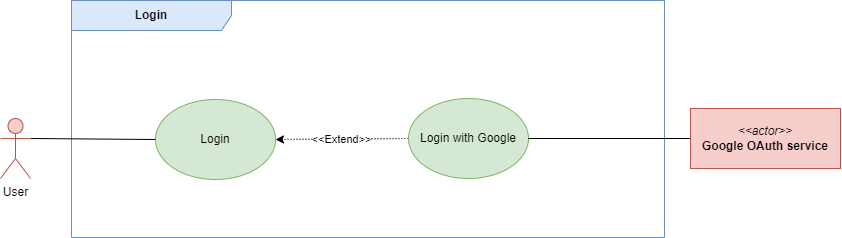
\includegraphics[width=0.7\textwidth]{Figures/login_ucd.png}
  \caption{Use-case diagram of the login function}
  \label{fig:login_activity_diagram}
\end{figure}

\begin{longtblr}[
    caption = {Use Case: Log In},
    label = {tblr:login_use_case},
  ]{
    vline{1-16} = {-}{},
    hline{-} = {1-2}{},
    colspec={X[3,l] X[7, l]},
  }
  \textbf{Use-case name} & \textbf{Log in} \\
  \textbf{Actors} & {
    User, Google OAuth Service
  } \\
  \textbf{Preconditions} & {
    User at login page
  } \\
  \textbf{Postconditions} & {
    Users log in successfully and can access authorized features.
  } \\
  \textbf{Triggers} & {
    1. Users access any authorized features of the system without being authorized.
    \\2. Users want to log in to the system.
  } \\
  \textbf{Normal flow} & {
    1. Users click on the login button of the system. The system displays a login form screen.
    \\2. User provides authentication information including email and password.
    \\3. The system verifies the authentication information.
    \\4. System grants access permission to users.
  } \\
  \textbf{Alternative flows} & {
    Alternative flow 1, at step 1:
    \\1. Users access any authorized features of the system without being authorized.
    \\Alternative flow 2:
    \\1. Users choose the option of login with a Google account. The system displays a Google login form screen.
    \\2. Users provide Google authentication information.
    \\3. Google Auth service verifies the authentication information and generates access tokens.
    \\4. System validates access token and grants access permission to users.
  } \\
  \textbf{Exceptions} & {
    1. Users input the wrong authentication information.
    \\2. Users do not have an account.
    \\3. Users do not have a Google account.
    \\4. Google OAuth Service works incorrectly.
  } \\
\end{longtblr}


\subsection{Register}

\begin{longtblr}[
    caption = {Use Case: Register},
    label = {tblr:register_use_case},
  ]{
    vline{1-13} = {-}{},
    hline{-} = {1-2}{},
    colspec={X[3,l] X[7, l]},
  }
  \textbf{Use-case name} & \textbf{Register} \\
  \textbf{Actors} & {
    User
  } \\
  \textbf{Preconditions} & {
    Users at register page
  } \\
  \textbf{Postconditions} & {
    Users register new accounts successfully
  } \\
  \textbf{Triggers} & {
    Users want to create new accounts and can access authorized features
  } \\
  \textbf{Normal flow} & {
    1. Users click on the register button of the system. The system displays a register form screen.
    \\2. Users provide authentication information (including email and password) and other personal information.
    \\3. The system verifies register information and sends validation emails to users.
    \\4. Users click on the link in the validation emails. The system creates new accounts and grants access permission to the guests (now become users).
  } \\
  \textbf{Alternative flows} & {
    Alternative flow 1, from step 3:
    \\3. System verifies provided information as invalid and rejects the registration.
  } \\
  \textbf{Exceptions} & {
    1. Provided emails are already in use.
    \\2. Guests do not confirm the validation email on time.
  } \\
\end{longtblr}


\subsection{Update to organization account}

\begin{figure}[H]
  \centering
  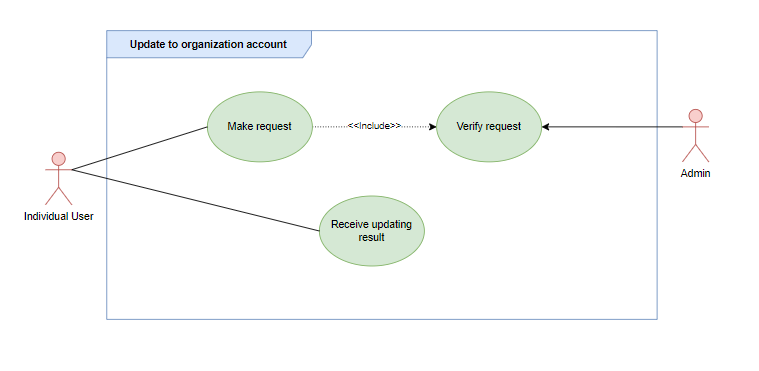
\includegraphics[width=0.7\textwidth]{Figures/update_org_ucd.png}
  \caption{Use-case diagram of the update to organization account function}
  \label{fig:update-org_activity_diagram}
\end{figure}

\begin{longtblr}[
    caption = {Use Case: Update To Organization Account},
    label = {tblr:update_organization_use_case},
  ]{
    vline{1-11} = {-}{},
    hline{-} = {1-2}{},
    colspec={X[3,l] X[7, l]},
  }
  \textbf{Use-case name}     & \textbf{Update to organization account} \\
  \textbf{Actors}            & {
      User, Admin.
  }                                                                    \\
  \textbf{Preconditions}     & {
      1. Admins have logged into the system.
  \\2. Users have an individual user account.
  }                                                                    \\
  \textbf{Postconditions}    & {
      Users update their account successfully.
  }                                                                    \\
  \textbf{Triggers}          & {
      1. Users logged into the systems.
  \\2. Users are on the user profile page.

  }                                                                    \\
  \textbf{Normal flow}       & {
      1. Users choose to update to organization accounts.
  \\2. Users provide some information for verification and submit them.
  \\3. Admins verify the update-account application.
  \\4. The system updates the accounts and notifies the user of the results.
  }                                                                    \\
  \textbf{Alternative flows} & {
      Alternative flow, from step 3:
  \\3. Admins decline the update applications.
  \\4. The system notifies the user of the results.
  }                                                                    \\
  \textbf{Exceptions}        & {

  }                                                                    \\
\end{longtblr}


\subsection{Mange pet profile}

\begin {figure}[H]
\centering
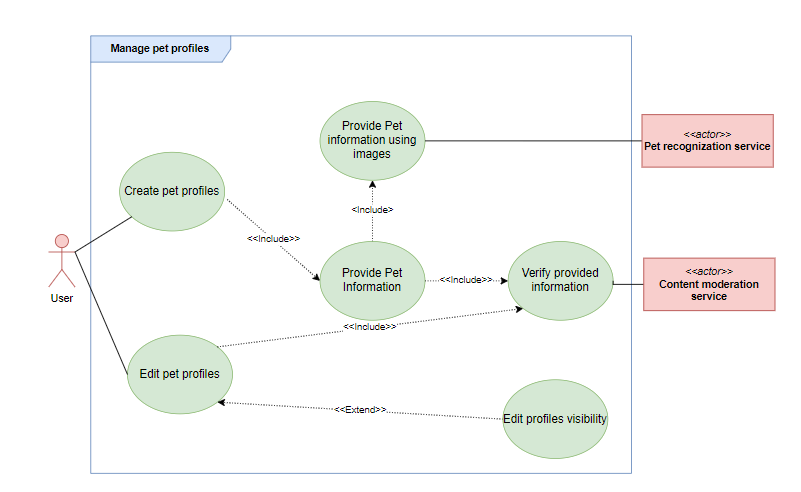
\includegraphics[width=0.7\textwidth]{Figures/manage_pet_ucd.png}
\caption{Use-case diagram of the manage pet profile function}
\label{fig:manage-pet-activity-diagram}
\end{figure}

\begin{longtblr}[
    caption = {Use Case: Manage Pet Profile},
    label = {tblr:manage_pet_profile_use_case},
  ]{
    vline{1-14} = {-}{},
    hline{-} = {1-2}{},
    colspec={X[3,l] X[7, l]},
  }
  \textbf{Use-case name}     & \textbf{Manage pet profile} \\
  \textbf{Actors}            & {
      User, Pet Recognization Service.
  }                                                        \\
  \textbf{Preconditions}     & {
      Users logged successfully into the system.
  }                                                        \\
  \textbf{Postconditions}    & {
      Users create and edit their pet profiles successfully.
  }                                                        \\
  \textbf{Triggers}          & {
      Users access the pet profile management section of the system.
  }                                                        \\
  \textbf{Normal flow}       & {
      1. Users click on the add profiles button of the system. The system displays a form screen of a pet profile.
  \\2. Users input their pet images. Pet Recognition Service automatically fills breed and color fields.
  \\3. Users fill in the remaining fields and submit.
  \\4. The system verifies submitted information using the Content Moderation service.
  \\5. The system creates new pet profiles and notifies the users.
  }                                                        \\
  \textbf{Alternative flows} & {
      Alternative flow 1, from step 2 to step 3:
  \\2. Users input the forms manually.
  \\Alternative flow 2, at step 3:
  \\3. Users edit input fields generated by Pet Recognization Service and submit.
  \\Alternative flow 3:
  \\1. Users choose their available pet profiles and click on the edit button. The system displays a form screen of pet profiles.
  \\2. Users edit and submit their pet information.
  \\3. The system updates the pet profiles and notifies the users.
  \\Alternative of flow 3, from step 2 of alternative flow 2:
  \\2. Users choose to remove their pet profiles. The system asks for confirmation.
  \\3. Users confirm removing pet profiles. The system deletes pet profiles and notifies users.
  }                                                        \\
  \textbf{Exceptions}        & {
      Pet Recognization Service cannot detect and fill in pet information.
  }                                                        \\
\end{longtblr}


\subsection{Access pet profile}

\begin {figure}[H]
\centering
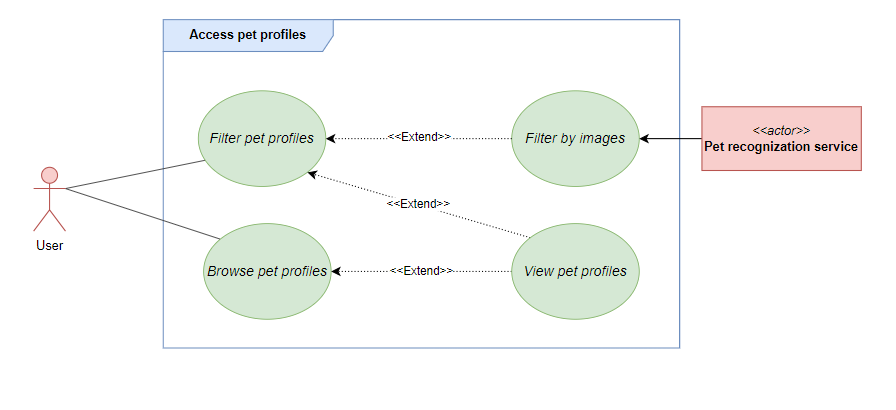
\includegraphics[width=0.7\textwidth]{Figures/access_pet_ucd.png}
\caption{Use-case diagram of the access pet profile function}
\label{fig:access-pet-activity-diagram}
\end{figure}

\begin{longtblr}[
    caption = {Use Case: Access Pet Profiles},
    label = {tblr:access_pet_profiles_use_case},
  ]{
    vline{1-11} = {-}{},
    hline{-} = {1-2}{},
    colspec={X[3,l] X[7, l]},
  }
  \textbf{Use-case name}     & \textbf{Access pet profiles} \\
  \textbf{Actors}            & {
      User
  }                                                         \\
  \textbf{Preconditions}     & {
      User at search page.
  }                                                         \\
  \textbf{Postconditions}    & {
      Users view their desired pets.
  }                                                         \\
  \textbf{Triggers}          & {
      Users access the system and want to find pets.
  }                                                         \\
  \textbf{Normal flow}       & {
      1. Users access the pet section. The system displays the pet section screen.
  \\2. Users select categories to filter. System filter and display list of pets.
  \\3. Users choose a pet profile. The system shows the pet profile details.
  }                                                         \\
  \textbf{Alternative flows} & {
      Alternative flow 1, from step 2:
  \\2. Users select a pet profile displayed in the pet section. The system shows the pet profile details.
  \\Alternative flow 2, from step 3:
  \\3. Users choose to filter by an image. The system sends the image to the pet recognition service.
  \\4. The service extracts information from images. System filter and display list of pets.
  \\5. Users choose a pet profile. The system shows the pet profile details.
  \\Alternative flow 3, at step 2
  \\2. Users filter pets by inputting text keywords.
  }                                                         \\
  \textbf{Exceptions}        & {
      1. The system does not have the user’s desired pet.
  \\2. The pet recognition service cannot extract information from the provided image.
  }                                                         \\
\end{longtblr}


\subsection{Adopt pets}

\begin {figure}[H]
\centering
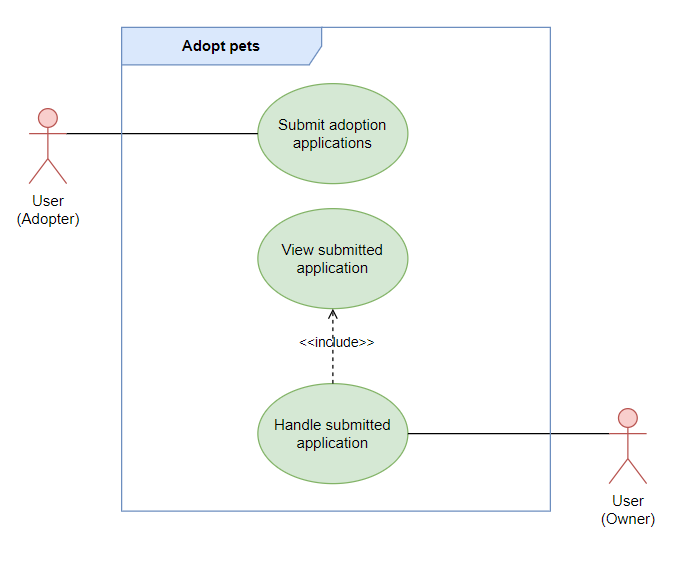
\includegraphics[width=0.7\textwidth]{Figures/adopt_pet_ucd.png}
\caption{Use-case diagram of the adopt pets function}
\label{fig:adopt-pet-activity-diagram}
\end{figure}

\begin{longtblr}[
    caption = {Use Case: Adopt pets},
    label = {tblr:adopt_pets_use_case},
  ]{
    vline{1-12} = {-}{},
    hline{-} = {1-2}{},
    colspec={X[3,l] X[7, l]},
  }
  \textbf{Use-case name} & \textbf{Adopt pets} \\
  \textbf{Actors} & {
    General User
  } \\
  \textbf{Preconditions} & {
    1. Users logged successfully into the system.
    \\2. Pet Adopters find pet profiles successfully.
  } \\
  \textbf{Postconditions} & {
    Pet owners receive and handle the submitted application successfully.
  } \\
  \textbf{Triggers} & {
    The adopters choose a pet profile and want to adopt.
  } \\
  \textbf{Normal flow} & {
    1. Pet adopters click the adopt button on a pet profile. The system displays a form screen of required information.
    \\2. Pet adopters fill required information and apply.
    \\3. Pet Owners receive and view the applications.
    \\4. Pet Owners accept the applications.
    \\5. The system updates the pet profile status and notifies the pet adopter of the results of the applications.
  } \\
  \textbf{Alternative flows} & {
    Alternative flow 1, from step 3:
    \\3. Pet adopters cancel their applications before Pet Owners accept them.
    \\Alternative flow 2, from steps 4 to 5:
    \\4. Pet Owners decline the applications.
    \\5. The system notifies pet adopters of the results of the applications.
  } \\
  \textbf{Exceptions} & {
    1. The pets already have new owners during the adoption process.
\\2. Pet adopters already sent a form before.

  } \\
\end{longtblr}


\subsection{Create posts}

\begin{longtblr}[
    caption = {Use Case: Create Posts},
    label = {tblr:create_posts},
  ]{
    vline{1-14} = {-}{},
    hline{-} = {1-2}{},
    colspec={X[3,l] X[7, l]},
  }
  \textbf{Use-case name}     & \textbf{Create posts}                  \\
  \textbf{Actors}            & User                                   \\
  \textbf{Preconditions}     & {
      1. User successfully adopted at least one pet.
  \\2. User has created a pet profile.
  }                                                                   \\
  \textbf{Postconditions}    & User creates pet posts successfully.   \\
  \textbf{Triggers}          & {
    1. Users update their adopted pet status. \\
    2. Users want to create pet posts
  }\\
  \textbf{Normal flow}       & {
      1. Users choose a profile of an adopted pet.
  \\2. Users click on the update status button of the pet profile. The system displays a form screen of update-status posts.
  \\3. Users input content for the post (including text and images) and submit.
  \\4. The system creates a new post and notifies pet adopters, pet owners, and admins.
  }                                                                   \\
  \textbf{Alternative flows} &                                        \\
  \textbf{Exceptions}        &                                        \\
\end{longtblr}


\subsection{Interact with pet posts}

\begin{longtblr}[
    caption = {Use Case: Interact with pet posts},
    label = {tblr:interact_with_pet_posts_use_case},
  ]{
    vline{1-9} = {-}{},
    hline{-} = {1-2}{},
    colspec={X[3,l] X[7, l]},
  }
  \textbf{Use-case name} & \textbf{Interact with pet posts} \\
  \textbf{Actors} & {
    General User
  } \\
  \textbf{Preconditions} & {
    1. Users logged successfully into the system.
    \\2. Users access a pet profile successfully.
    \\3. The pet is adopted and has at least one status-update blog uploaded.
  } \\
  \textbf{Postconditions} & {
    Users can interact with pet posts.
  } \\
  \textbf{Triggers} & {
    Users choose to view an adopted pet profile.
  } \\
  \textbf{Normal flow} & {
    1. Users access update-status posts. The system displays an update-status posts screen.
    \\2. Users view the content of the post.
    \\3. Users like the post by using the like option.
    \\4. System updates the update-status posts.
  } \\
  \textbf{Alternative flows} & {
    Alternative flow 1, at step 3:
    \\3. Users leave comments in the comment section of the blog.
  } \\
  \textbf{Exceptions} & {
    Pet posts will not appear if they are private and the users do not have an appropriate role to view them.
  } \\
\end{longtblr}

\subsection{Make payement}

\begin {figure}[H]
\centering
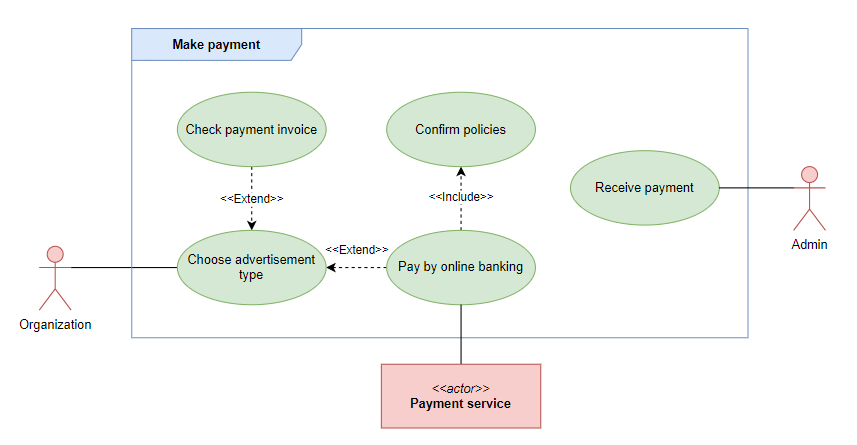
\includegraphics[width=0.7\textwidth]{Figures/payment_ucd.png}
\caption{Use-case diagram of the make payment function}
\label{fig:payment-activity-diagram}
\end{figure}


\begin{longtblr}[
    caption = {Use Case: Make payment},
    label = {tblr:make_payment_use_case},
  ]{
    vline{1-10} = {-}{},
    hline{-} = {1-2}{},
    colspec={X[3,l] X[7, l]},
  }
  \textbf{Use-case name} & \textbf{Make payment} \\
  \textbf{Actors} & {
    Organization, Admin, Payment service
  } \\
  \textbf{Preconditions} & {
    Organizations create a blog successfully.
  } \\
  \textbf{Postconditions} & {
    1. Organizations have blogs that have the correct advertisement duration.
    \\2. Admins receive payment from organizations.
  } \\
  \textbf{Triggers} & {
    Organizations apply advertisements on their blogs.
  } \\
  \textbf{Normal flow} & {
    1. The system shows all advertisement types with their periods.
    \\2. Users choose a type of advertisement. The system shows the payment invoice.
    \\3. Users confirm all the payment policies and finish the payments.
    \\4. Payment service processes the transactions.
    \\5. Admins receive the payments from the organizations.
    \\6. System notifies organizations and admins of successful payments.
  } \\
  \textbf{Alternative flows} & {
    Alternative flow 1, at step 3:
    \\3. Users can refuse the payment policies and stop the payments.
    \\Alternative flow 2, from step 4:
    \\4. Payment service processes the transactions and gets errors.
    \\5. System notifies organizations of failed payments.
  } \\
  \textbf{Exceptions} & {
    1. Organizations do not use the supported payment service.
    \\2. The balances in the accounts of organizations are not enough.
    \\3. Internal errors in the payment service occur.
  } \\
\end{longtblr}


\subsection{Manage blogs}

\begin {figure}[H]
\centering
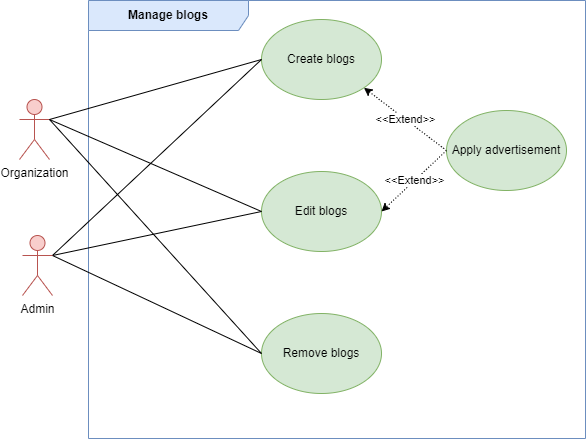
\includegraphics[width=0.7\textwidth]{Figures/manage_blog_ucd.png}
\caption{Use-case diagram of the manage blogs function}
\label{fig:manage-blog-activity-diagram}
\end{figure}

\begin{longtblr}[
    caption = {Use Case: Manage Blogs},
    label = {tblr:manage_blogs},
  ]{
    vline{1-14} = {-}{},
    hline{-} = {1-2}{},
    colspec={X[3,l] X[7, l]},
  }
  \textbf{Use-case name}     & \textbf{Manage blogs}                                           \\
  \textbf{Actors}            & Organization, Admin                                             \\
  \textbf{Preconditions}     & Organizations logged successfully into the system.              \\
  \textbf{Postconditions}    & Organizations can create and edit their blogs.                  \\
  \textbf{Triggers}          & Organizations access the blog management section of the system. \\
  \textbf{Normal flow}       & {
      1. Organizations click on the add blogs button of the system. The system displays a blog form screen.
  \\2. Organizations provide and submit blog creation forms.
  \\3. The system creates new blogs.
  }                                                                                            \\
  \textbf{Alternative flows} & {
      Alternative flow 1: from step 1:
  \\1. Organizations choose to update blogs. The system displays a blog form screen.
  \\2. Organizations provide and submit blog update forms.
  \\3. The system updates the blogs.
  \\Alternative flow 2 (for both normal flow and flow 1), from step 3:
  \\4. Organizations apply advertisement on blogs.
  \\5. The system updates the blogs to advertisement blogs.
  }                                                                                            \\
  \textbf{Exceptions}        &                                                                 \\
\end{longtblr}


\section{Workflow analysis}
\subsection{Activity Diagrams}

\subsubsection{Self Registration}

The use case starts when a user accesses the register page (or clicks the register button on the login form), and then a register form will be displayed. The user provided some information (including email, password, and name). Then,  the provided information is verified. If it is valid, a confirmation email will be sent to the user. After accessing the link in the email, a new account is created and the user can log into the system.

\begin{figure}[H]
  \centering
  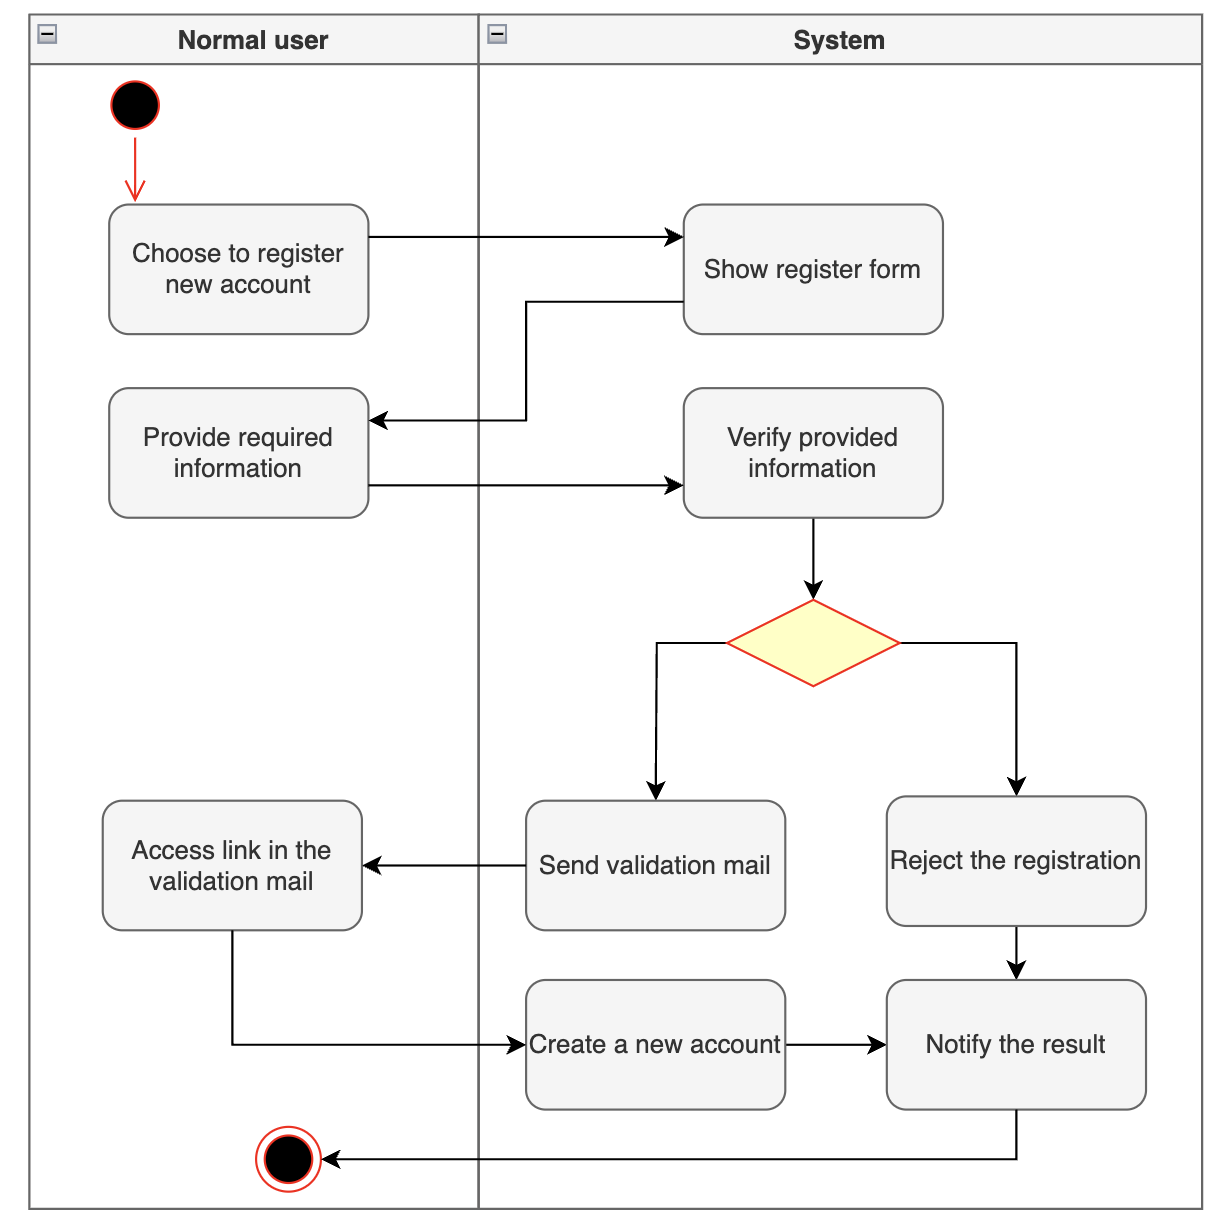
\includegraphics[width=0.7\textwidth]{Figures/self_register.png}
  \caption{Self Registration activity diagram}
  \label{fig:self-registration}
\end{figure}


\subsubsection{Login}

The use case starts when an unauthorized user tries to access internal features or goes to the login page. The user at the login can provide an email and password and send them to the system. If the credential information is valid, the user will be granted access permission and navigated to an internal page. Otherwise, an error alert will be displayed.

\begin{figure}[H]
  \centering
  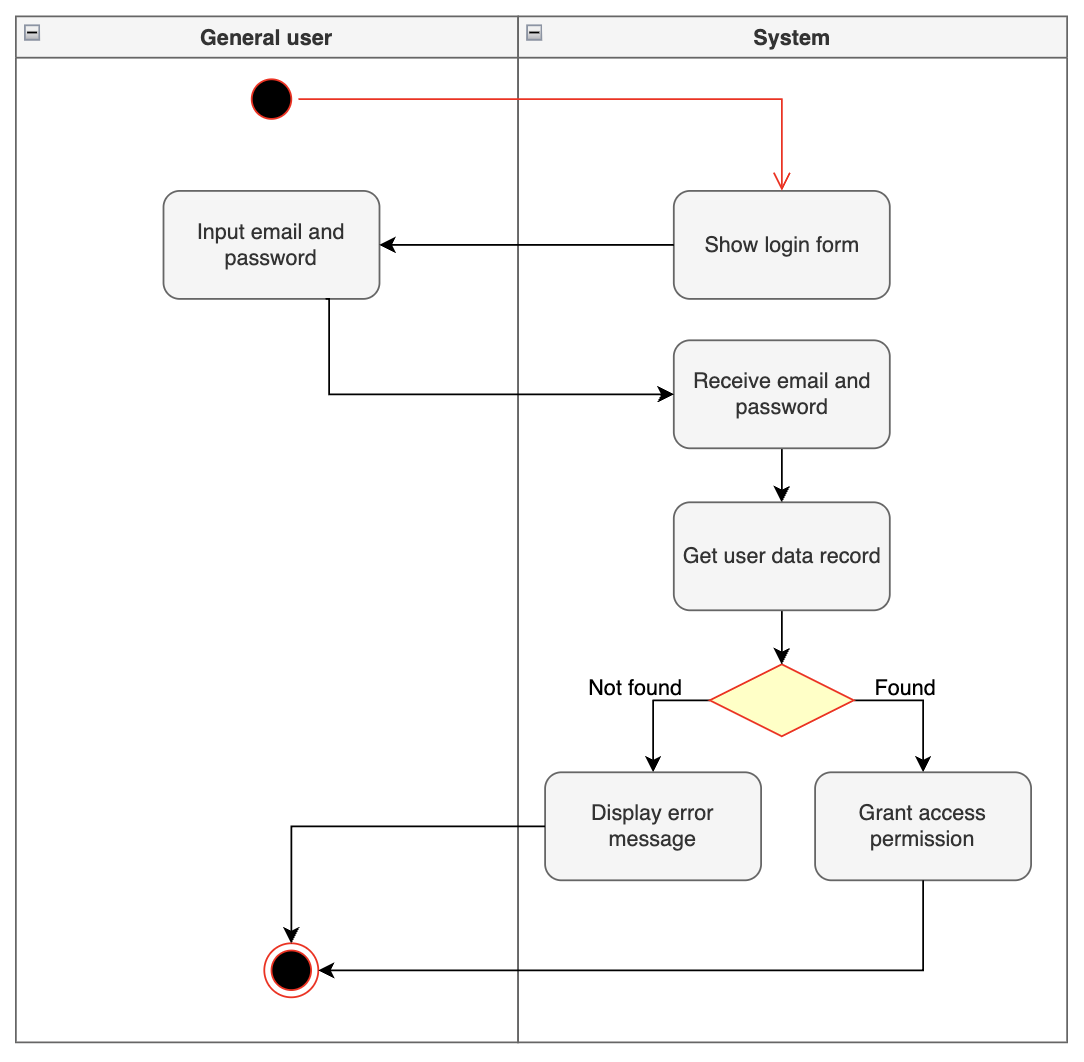
\includegraphics[width=0.7\textwidth]{Figures/login.png}
  \caption{Login activity diagram}
  \label{fig:login}
\end{figure}

\subsubsection{Login with a Google account}

The use case starts when a user chooses the option of logging in with a Google account, then a Google login form will be displayed. Users provide Google authentication information. Google Auth service verifies the authentication information and generates an access token. Finally, the system validates the access token and grants access permission to the user.

\begin{figure}[H]
  \centering
  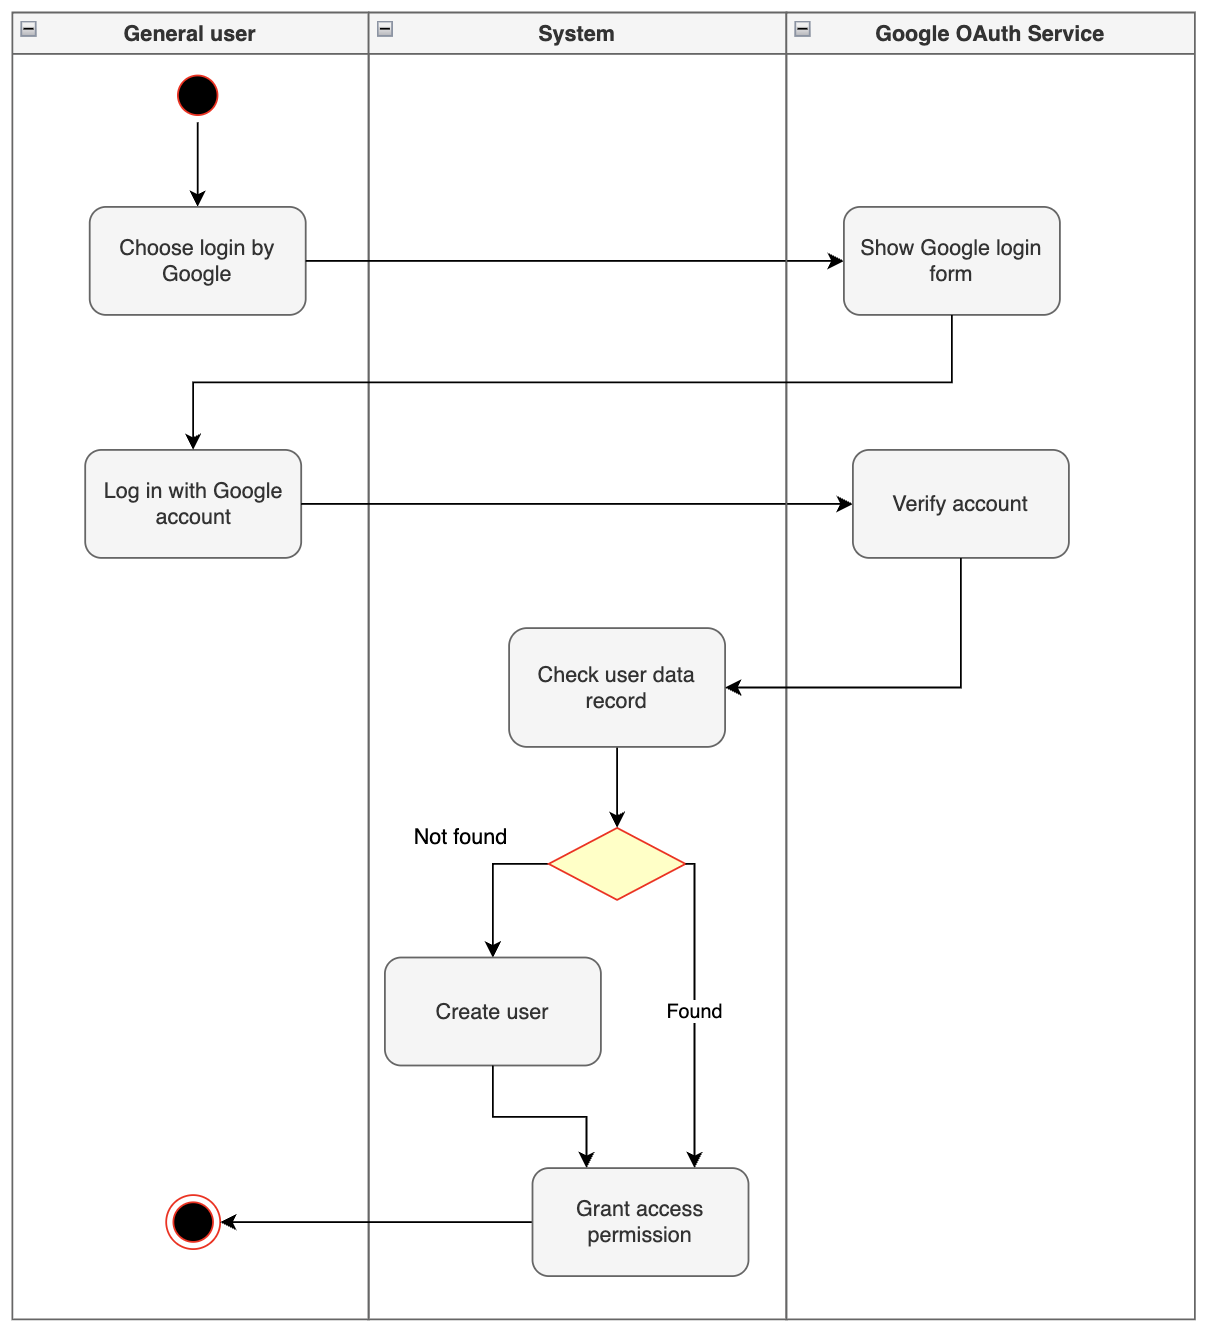
\includegraphics[width=0.7\textwidth]{Figures/login_gg.png}
  \caption{Login with a Google account activity diagram}
  \label{fig:login-google}
\end{figure}

\subsubsection{Update to Organization account}

The use case starts when an individual user chooses to update to organization accounts, then a form will be displayed. Then, users provide some information for verification and submit them. After the update-account application is verified by admins, the system updates the account and notifies the user of the results.

\begin{figure}[H]
  \centering
  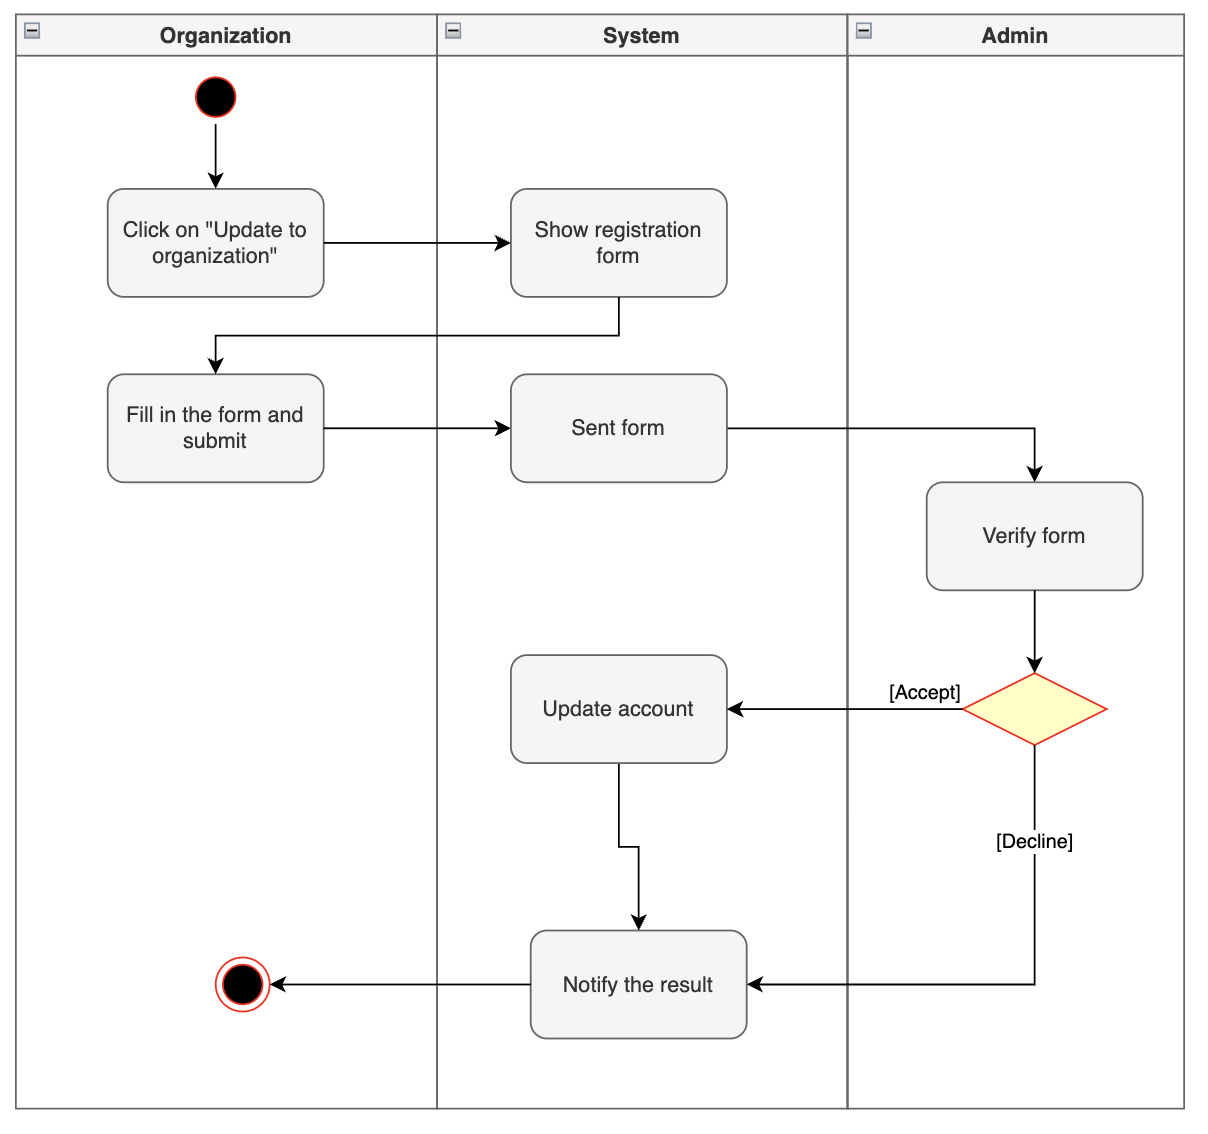
\includegraphics[width=0.7\textwidth]{Figures/update_org.png}
  \caption{Update to Organization account activity diagram}
  \label{fig:update-org}
\end{figure}

\subsubsection{Manage pet profiles}


\begin{figure}[H]
  \centering
  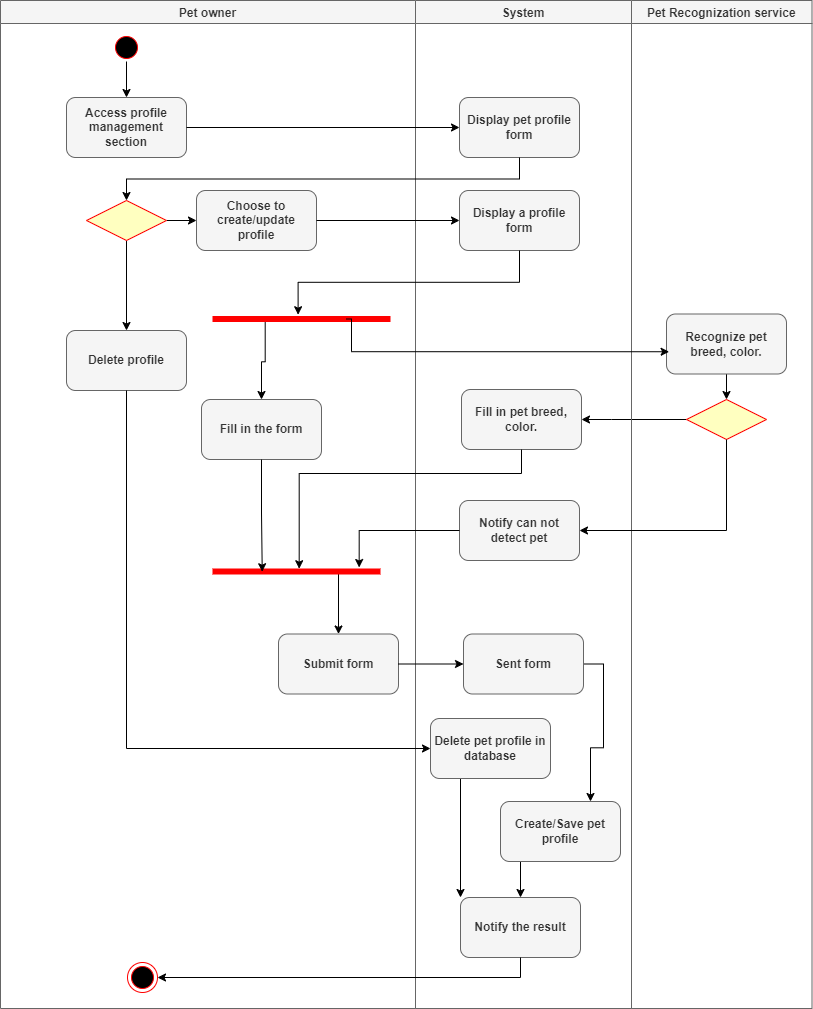
\includegraphics[width=0.7\textwidth]{Figures/manage_pet.png}
  \caption{Manage pet profile activity diagram}
  \label{fig:manage-pet}
\end{figure}

The use case starts when a user accesses the pet profile management page. The user chooses to edit or create a new profile and a form will be displayed. Note that the form would be filled if the user chose to edit an available profile. In that case, the user can modify the fields or rather delete the profile. Otherwise, the user can input the pet information and submit it. The user can also fill in pet breeds and colors by providing images. Finally, the content of the form will be verified, and the result will be displayed.


\subsubsection{Access pet profile}

In the pet profile page, a user has options to find pets by filtering by categories or providing pet images. In case the user filters by images, those images will be processed by the Pet Recognition Service. Then, the filtered pet profiles will be displayed to the user. The user can click on pet profiles for further information or continue finding other pet profiles.

\begin{figure}[H]
  \centering
  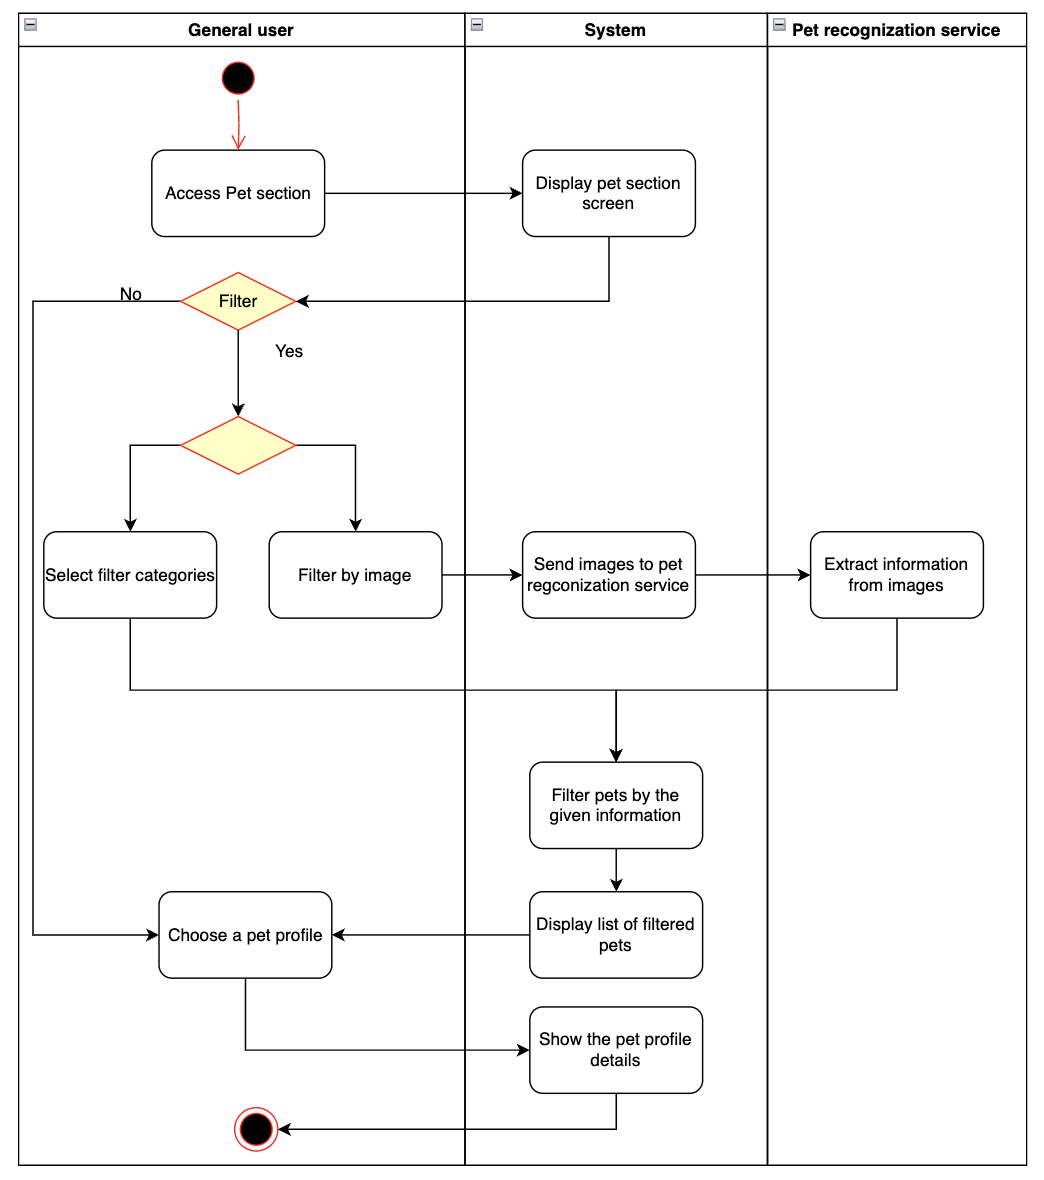
\includegraphics[width=0.7\textwidth]{Figures/access_pet.png}
  \caption{Access pet profile activity diagram}
  \label{fig:access-pet}
\end{figure}

\subsubsection{Adopt pets}

After finding a pet profile successfully, if the pet is still available, a user can choose to adopt the pet by filling in the required information in the adoption form and sending it. The application form will be reviewed by the pet owner. The result will be sent to the user then. Note that, the user can still contact directly to the pet owner during the pet adoption process.

\begin{figure}[H]
  \centering
  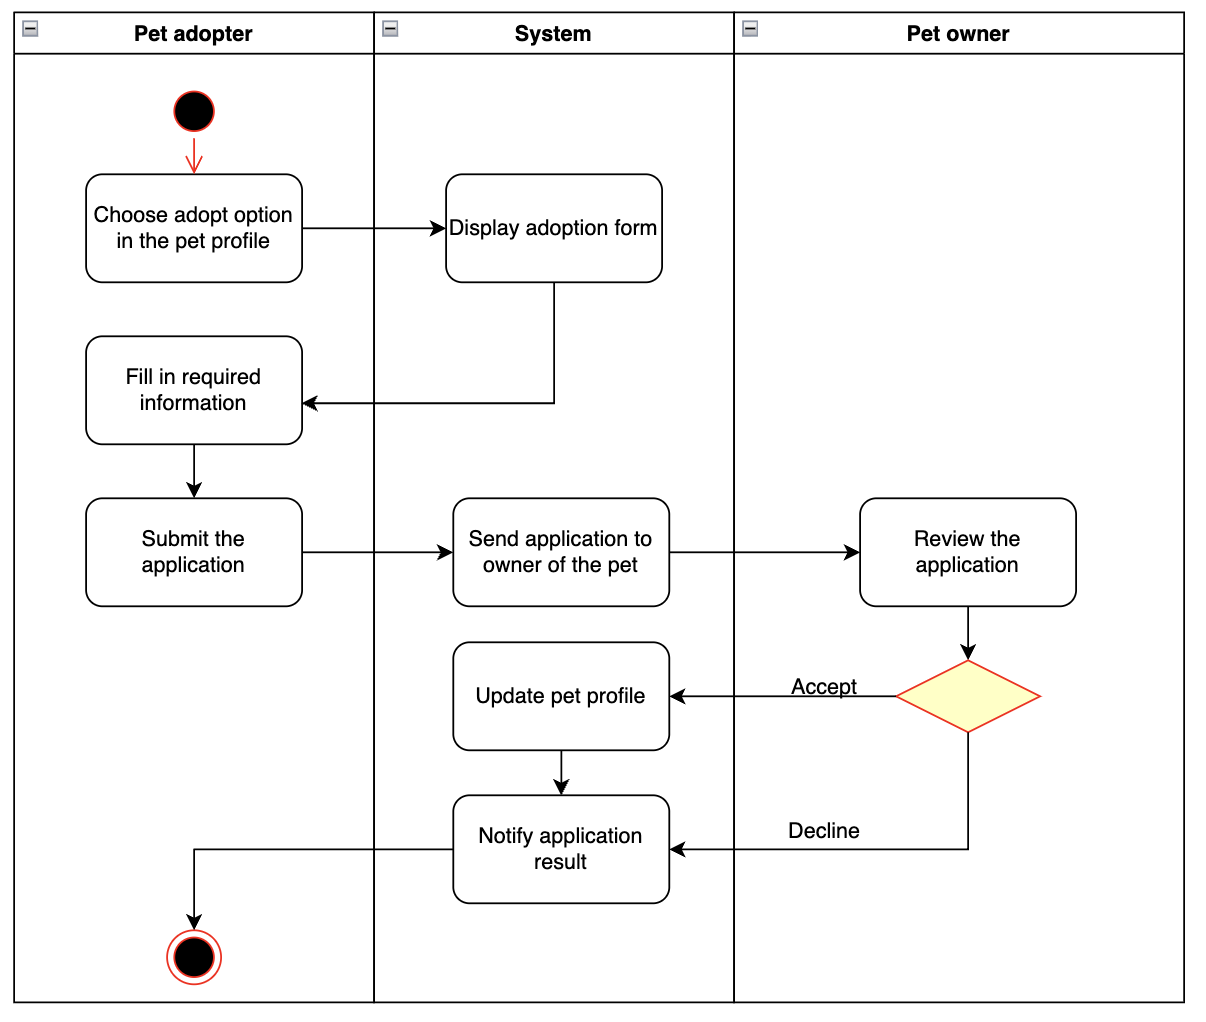
\includegraphics[width=0.7\textwidth]{Figures/adopt_pet.png}
  \caption{Adopt pets activity diagram}
  \label{fig:adopt-pet}
\end{figure}

\subsubsection{Interact with posts}

After accessing a pet profile successfully, a user can also see public posts of the pet. The user can choose a post for further information and leave their comments or likes on the post. Note that the private posts can only be seen by the pet owner and admins.

\begin{figure}[H]
  \centering
  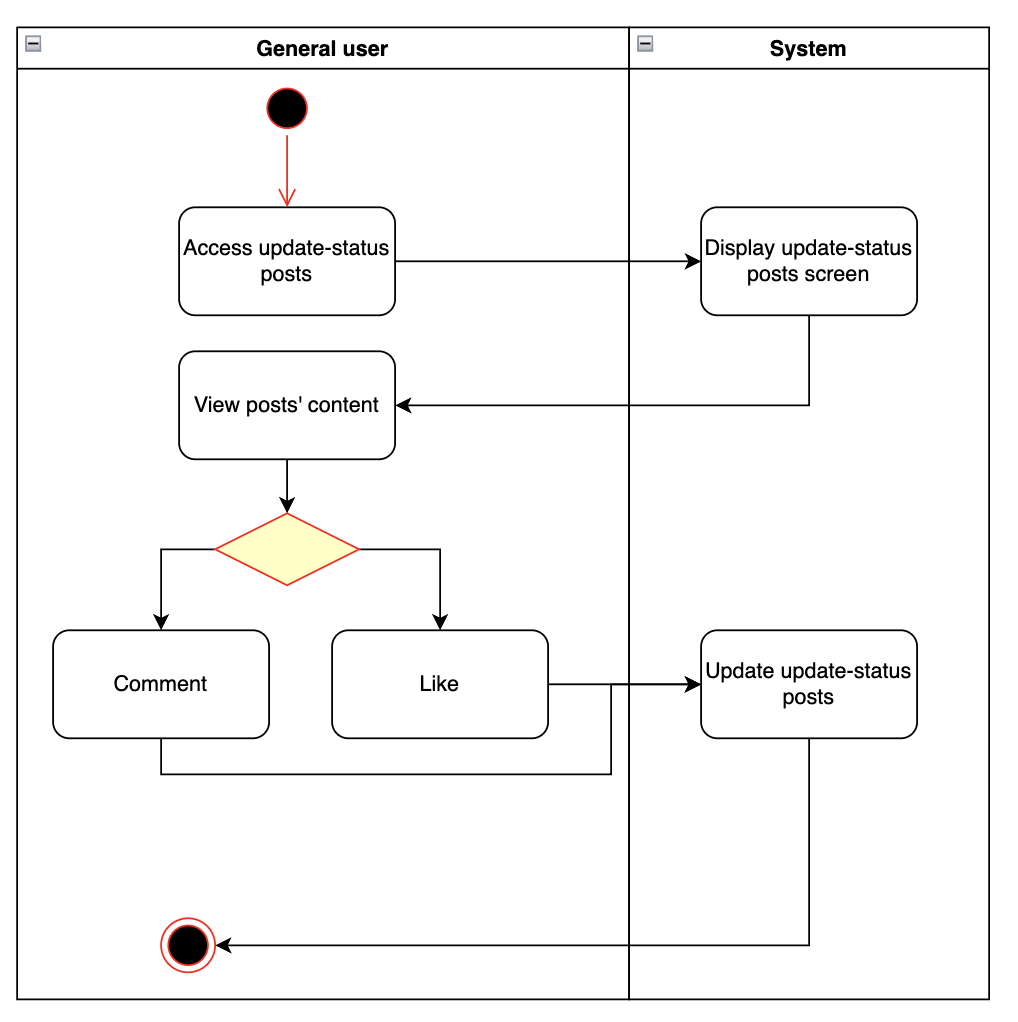
\includegraphics[width=0.7\textwidth]{Figures/post_interact.png}
  \caption{Interact with posts activity diagram}
  \label{fig:interact-post}
\end{figure}

\subsubsection*{Create posts}

\begin{figure}[H]
  \centering
  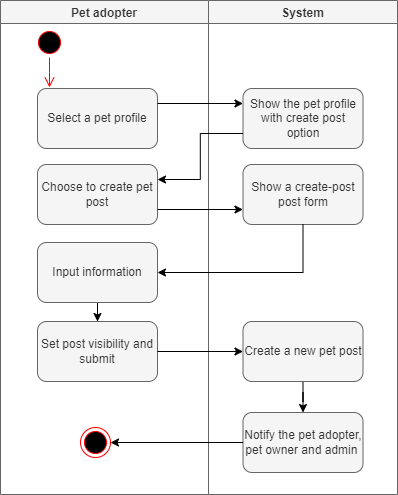
\includegraphics[width=0.7\textwidth]{Figures/create-pet-post.png}
  \caption{Create posts activity diagram}
  \label{fig:create-post}
\end{figure}

Updating the status of a pet is uploading posts about it. The use case starts when an owner can select a pet profile and choose the option of updating the pet status. After filling information, the owner can set visibility for the post. Finally, the user can send the form and a new post is created.


\subsubsection{Manage blogs}

The use case starts when a user with an Organization account accesses the blog management page. The user chooses to edit or create a new blog, then a form will be displayed. Note that the form would be filled if the user chose to edit an available blog. In that case, the user can modify the fields or rather delete the blog. If the user wants to create a new blog, the user can input and submit it. Finally, admins will verify the blog and the result will be sent to the user.

\begin {figure}[H]
\centering
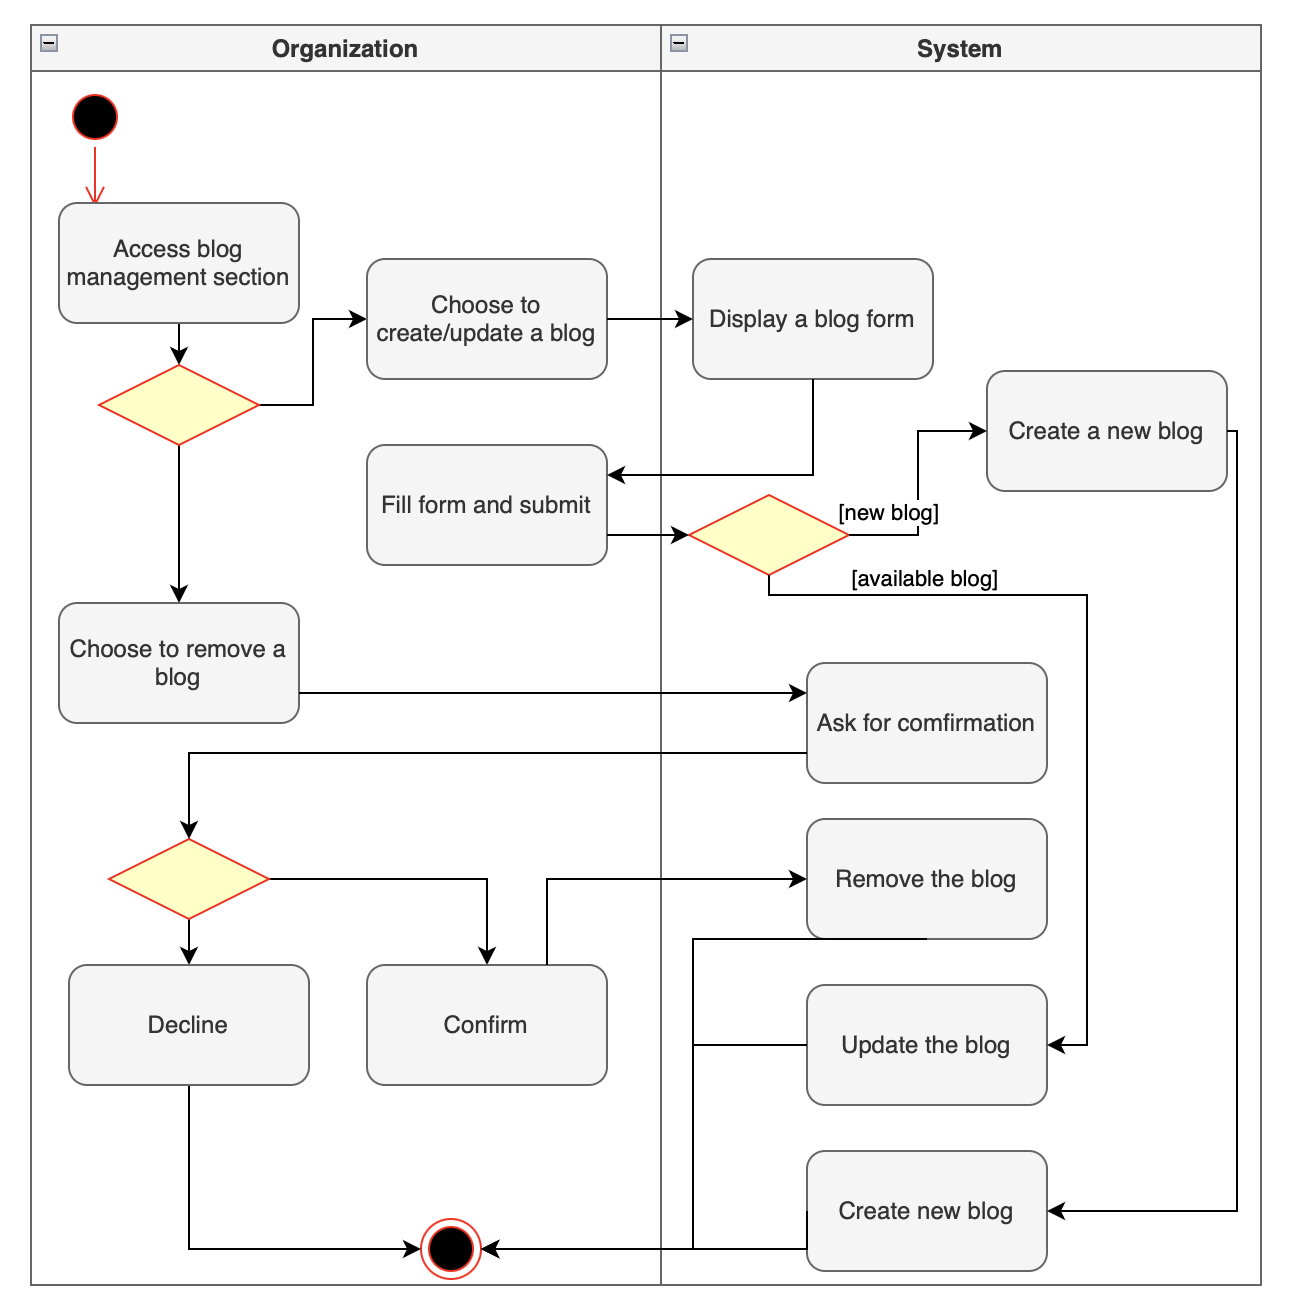
\includegraphics[width=0.7\textwidth]{Figures/manage_blog_org.png}
\caption{Manage blogs activity diagram}
\label{fig:manage-blog}
\end{figure}


\subsubsection{Make payment}

When a user applies an advertisement on a log, the system shows all advertisement types with their periods. Then, users choose a type of advertisement and the system shows the payment invoice. If the user confirms the payment, the Payment service will process the transaction and the result will be displayed to admins and the user.

\begin {figure}[H]
\centering
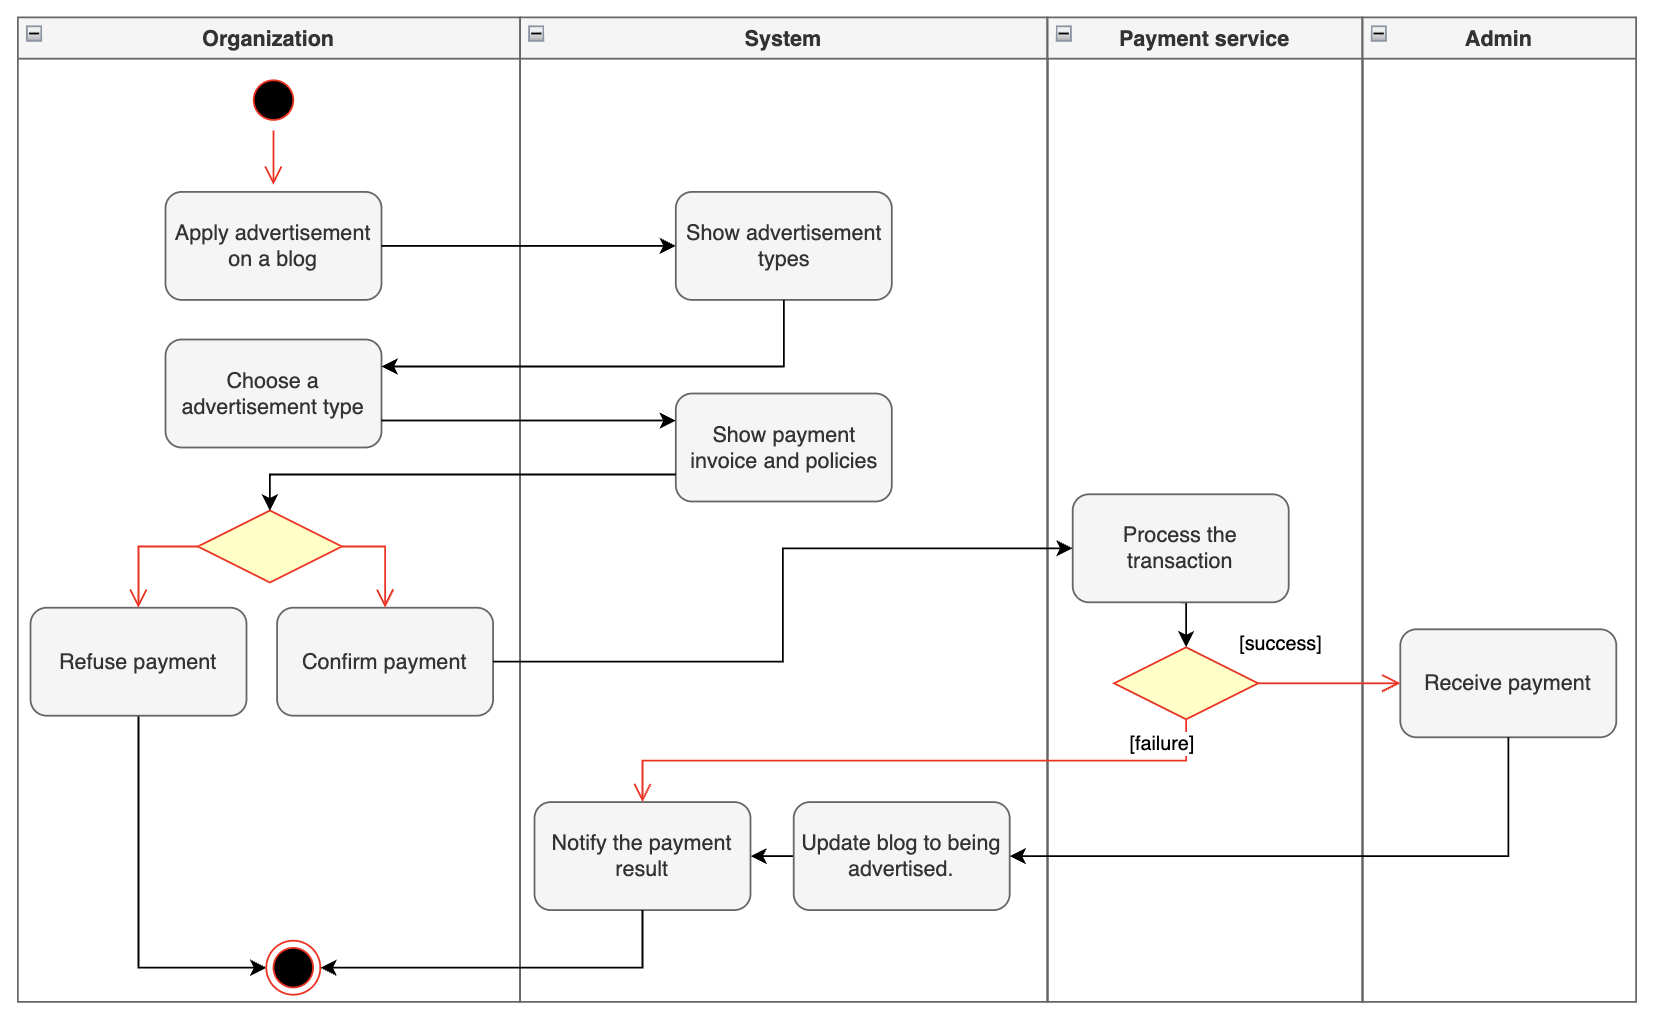
\includegraphics[width=0.7\textwidth]{Figures/payment.png}
\caption{Make payment activity diagram}
\label{fig:make-payment}
\end{figure}